
Population processes are processes that change the model state. These processes produce changes in the partition by adding or removing individuals, or by moving individuals between ages and/or categories.

Current population processes available include:

\begin{itemize}
\item recruitment\index{Recruitment} (Section~\ref{sec:Process-Recruitment}),
\item ageing\index{Ageing} (Section~\ref{sec:Process-Ageing}),
\item growth\index{Growth} (Section~\ref{sec:AgeLength}),
\item maturation\index{Maturation} (Section~\ref{sec:Process-TransitionCategory}),
\item mortality\index{Mortality} events (e.g., natural and fishing) (Section~\ref{sec:Process-Mortality}), 
\item category transition processes\index{Category transition}, i.e., processes that move individuals between categories while preserving their overall age structure (Section~\ref{sec:Process-TransitionCategory}), and
\item tagging and tag loss (Section~\ref{sec:Process-TagByAge}).
\end{itemize}

There are two types of processes: (1) processes that occur across multiple time steps in the annual cycle, e.g., \subcommand{mortality\_constant\_rate} and \subcommand{mortality\_instantaneous}; and (2) processes that occur only within the time step in which they are specified.

\subsubsection{\I{Recruitment}}\label{sec:Process-Recruitment}

Recruitment processes  add new individuals to the partition. Recruitment depends on virgin biomass or alternatively recruitment in the virgin state and so these parameters are located in this process (as \textit{b0} and \textit{r0}). The other factors needed are SSB if there is a stock-recruitment relationship and the CV for the prior on YCS (the mean is mandated to be 1 over some specified year range). Thus, a SSB label may have to be included (pointing to a derived quantity).

In the recruitment processes, a number of individuals are added to a single age class (subcommand \textit{age}) within the partition, with the number determined by the type of stock-recruitment process specified. If recruits are added to more than one category, then the proportion of recruits to be added to each category is specified by the \argument{proportions} subcommand. For example, if recruiting to categories labelled \texttt{male} and \texttt{female}, then the proportions may be set to $0.5$ and $0.5$, so that half of the recruits are added to the male category and the other half to the female category.

Recruitment can differ between a spawning event or the creation of a cohort/year class. One view for fisheries is that recruitment usually refers to individuals "recruiting" to a fishery. This definition is used because there is usually not a lot of information on younger age classes between the time of spawning and being vulnerable to a survey or fishery for data collection. However, here, recruitment is to a fixed age class for one or more categories.

The offset between spawning and recruitment is parametrised either by the recruitment subcommand \texttt{age}, or \texttt{min\_age}, which is the default value for the \texttt{age} subcommand in the recruitment process. The \CNAME\ parameter \texttt{age} is the same as the CASAL parameter \texttt{y\_enter}.\TODO{Check this} Notice that the minimum age is usually different from zero and so there is usually  a one or more year's delay between spawning and recruitment into the partition. There is also a complication from when spawning occurs in the annual cycle and when recruitment occurs.

\CNAME\ has two  recruitment processes, constant recruitment\index{Recruitment ! Constant} and the \I{Beverton-Holt stock-recruitment relationship}\index{Recruitment ! Beverton-Holt} \citep{1203}. The  number of individuals following recruitment in year $y$ is

\begin{equation}
N_{y,a,j} \leftarrow N_{y,a - 1,j} + p_j(R_y)
\end{equation}

where $N_{y,a,j}$ is the numbers in year $y$ and category $j$ at age $a$, $p_j$ is the proportion added to category $j$, and $R_y$ is the total number of recruits in year $y$.

\paragraph{\I{Constant recruitment}}\label{sec:Process-RecruitmentConstant}

In the constant recruitment process the total number of recruits added in each year $y$ in age $a$ is $R_y$, with $R_y = R_0$ for all years

\begin{equation}
  R_{y,j} = p_j(R_0)
\end{equation}

Constant recruitment is equivalent to a Beverton-Holt recruitment process with steepness ($h$) set to 1.

For example, to specify a constant recruitment process where individuals are added to the male and female immature categories at $age=1$ in equal proportion (\texttt{proportions} = 0.5), and the number to add is $R_0=5 \times 10^5$, the syntax is

{\small{\begin{verbatim}
	@process Recruitment
	type constant_recruitment
	categories male.immature female.immature
	proportions 0.5 0.5
	r0 500000
	age 1
\end{verbatim}}}

\paragraph{\I{Beverton-Holt recruitment}}\label{sec:Process-RecruitmentBevertonHolt}

In the Beverton-Holt recruitment process the total number of recruits added each year is $R_y$. $R_y$ is the product of the average recruitment $R_0$, the annual year class strength multiplier $YCS$, and the stock-recruit relationship $SR(SSB_y)$

\begin{equation}\label{eq:BH}
  R_{y,a,j} = p_j(R_0 \times YCS_{ycs\_year} \times SR(SSB_{ycs\_year}))
\end{equation}

where

\begin{equation}\label{eq:year_class}
ycs\_year = y - \texttt{ssb\_offset}
\end{equation}

and $a$ is age, $p_j$ is the proportion of recruits to enter category $j$, and \texttt{ssb\_offset} is the number of years lag between spawning and recruitment.

Recruitment refers to recruitment into the population and may differ from the spawning event. See below on more information about \texttt{ssb\_offset}. In general this parameter should not be specified by the user.

$SR(SSB_y)$ is the Beverton-Holt stock-recruit relationship parametrised by the steepness $h$, and based on \cite{mace_doonan_88} parametrisation

\begin{equation}\label{eq:BH_SR}
SR(SSB_y) = \frac{SSB_y}{B_0} / \left( 1-\frac{5h-1}{4h} \left( 1-\frac{SSB_y}{B_0} \right) \right)
\end{equation}

The Beverton-Holt recruitment process requires a value for \Bzero\ and $SSB_y$ to calculate the number of recruits. A derived quantity (see Section \ref{sec:DerivedQuantity}) must be defined that provides the annual $SSB_y$ for the recruitment process. \Bzero\ is then defined as the value of the $SSB$ at the end of one of the initialisation phases, which is defined by the parameter \texttt{b0\_initialisation\_phase}.

During initialisation the $YCS$ multipliers are assumed to be equal to 1, and recruitment that happens in the initialisation phases that occur before and during the phase when \Bzero\ is determined are assumed to have steepness $h=1$ (i.e., in those initialisation phases, recruitment is equal to \Rzero).

Recruitment in the initialisation phases after the phase where \Bzero\ was determined are calculated using the Beverton-Holt stock-recruit relationship. \Rzero\ and \Bzero\ have a direct relationship when there are no density-dependent processes in the annual cycle. Models can thus be initialised using \Bzero\ or \Rzero.

An example of the specification of a Beverton-Holt recruitment process, where individuals are added to the category "immature" at $age=1$, and the number added is $R_0=5 \times 10^5$; \texttt{SSB\_derived\_quantity} is a derived quantity that specifies the total spawning stock biomass that contributed to the year class, with \Bzero\ the value of the derived quantity at the end of the initialisation phase labelled \texttt{phase1}; and $YCS$ are standardised to have mean one in the period 1995 to 2004, and recruits enter into the model two years following spawning

{\small{\begin{verbatim}
	@process Recruitment
	type recruitment_beverton_holt
	categories immature
	proportions 1.0
	r0 500000
	b0_initialisation_phase phase1
	steepness 0.75
	age 1
	ssb SSB_derived_quantity

\end{verbatim}}}

The property \texttt{ssb\_offset} should not be manually specified; \CNAME\ determines \texttt{ssb\_offset} by the order of ageing, recruitment, spawning, and the recruitment parameter \texttt{age}

\begin{itemize}
	\item if the annual time step order is recruitment, ageing, spawning, then \texttt{ssb\_offset} should equal \texttt{age} + 1, or
	\item if the annual time step order is spawning, ageing, recruitment, then \texttt{ssb\_offset} should equal \texttt{age} - 1, or
	\item \texttt{ssb\_offset} = \texttt{age}
\end{itemize}

There may be scenarios where the user will input these values, e.g., if there are multiple ageing processes in the annual cycle. \CNAME\ does not have functionality to accommodate this situation, so in this case \texttt{ssb\_offset} would be manually defined.

There are two variants of this process and they refer to how the stock recruitment residuals or $YCS_{ycs\_year}$ are parametrised. This parametrisation can either be in natural space as year class strength ($YCS$) multipliers, or in log space as recruitment deviations. Due to the difference in terminology, these variants are implemented in two separate processes, \subcommand{type recruitment\_beverton\_holt} and \subcommand{type recruitment\_beverton\_holt\_with\_deviations}, respectively.

\paragraph*{YCS ($YCS_y$)}

The $YCS$ parameter (\texttt{ycs\_years}) is defined in Equation~\eqref{eq:year_class}. The parameter \texttt{ycs\_values} is referenced by the \texttt{ycs\_years} parameter and is important to note when defining \command{estimate}, \command{project}, and \command{time\_varying} blocks for the parameter \texttt{ycs\_values}. An example is at the end of the section.

A common practice when estimating $YCS$ is to standardise using the Haist parametrisation, which was described by V. Haist. \CNAME\ will standardise $YCS$ only if subcommand \subcommand{standardise\_ycs\_years} is defined. The model parameter \texttt{ycs\_values} is a vector \textbf{Y}, covering the years from \texttt{start\_year} - \texttt{ssb\_offset} to \texttt{final\_year} - \texttt{ssb\_offset}, as defined by the parameter \texttt{ycs\_years}. The resulting year class strengths are calculated by $YCS_i=Y_i/\bar{\textbf{Y}}$, where the mean is calculated over the user-specified years \texttt{standardise\_ycs\_years}.

An alternative to \enquote{standardisation} is to constrain the $YCS$ parameters using the simplex transformation (see Section~\ref{sec:Transformation-Simplex}). This is thought to have estimation benefits over the \enquote{standardisation} as priors can be applied to the \enquote{free} parameters (\(Y_i\)).

\[
YCS_i =
\begin{cases}
Y_i / mean_{y \in S}(Y_y) & :y \in S\\
Y_i					 & :y \notin S
\end{cases}
\]

where S is the set of years from \texttt{standardise\_ycs\_years}. One effect of this parametrisation is that \Rzero\ is then defined as the mean estimated recruitment over the set of years $S$, because the mean $YCS$ multiplier over these years will always be one.

Typically \texttt{standardise\_ycs\_years} is defined to span the years over which $YCS$ is reasonably well estimated. For years that are not well estimated, $Y_y$ can be set to 1 for some or all years $y\in S$ (which is equivalent to forcing $R_y$ = \Rzero\ x $SR(SSB_y)$) by setting the lower and upper bounds of these $Y$ values to 1. An exception to this might occur for the most recent $YCS$ values, which the user may estimate but not include in the definition of \Rzero\ (because the estimates may be based on too few data). One or more years may be excluded from the range of years for the averaging process of the Haist parametrisation.

The advantage of the Haist parametrisation is that a large penalty is not necessary to force the mean of the $YCS$ parameter to be 1, although a small penalty should still be used to stop the mean of \textbf{Y} from drifting. These adjustments may improve MCMC performance. Projected $YCS$ values are not affected by this feature. A disadvantage with this parametrisation in a Bayesian analysis is that the prior applies to $Y$, not $YCS$.

In the  example given above,  $YCS$ are standardised to have mean one in the period 1995 to 2004, and recruits enter into the model two years following spawning

{\small{\begin{verbatim}
	@process Recruitment
	type recruitment_beverton_holt
	...            #subcommand above
	standardise_ycs_years 1995:2004
	ycs_years  1994 1995 1996 1997 1998 1999 2000 2001 2002 2003 2004 2005 2006
	ycs_values 0.65 0.87  1.6 1.13 1.02 0.38 2.65 1.35    1    1    1    1    1
\end{verbatim}}}


\paragraph*{Recruitment deviations, $\epsilon_y$ (\emph{type recruitment\_beverton\_holt\_with\_deviations})} \label{sec:Process-RecruitmentBevertonHoltWithDeviations} \STATUS{Untested}

Recruitment deviations represent the stock-recruitment relationship residuals in log space, with the link between $YCS_y$ and $\epsilon_y$

\begin{equation}\label{eq:recruit_devs}
	YCS_y = exp(\epsilon_y - b_y\sigma^2_R / 2)
\end{equation}

where $\epsilon_y\sim N(0,\sigma^2_R)$, $\sigma^2_R$ is the variance of the stock-recruitment residuals, and $b_y$ is a bias correction defined by \cite{methot2011adjusting}

\begin{equation}\label{eq::bias}
b_y = \left\{\begin{array}{lr}
0, & \text{for }y\leq y_1^b\\
b_{max}(1 - \frac{y - y_1^b}{y_2^b - y_1^b}), & \text{for } y_1^b < y < y_2^b\\
b_{max}, & \text{for } y_2^b\leq y \leq y_3^b\\
b_{max}(1 - \frac{y_3^b - y}{y_4^b - y_3^b}), & \text{for }  y_3^b< y < y_4^b\\
0, & \text{for } y_4^b\leq y
\end{array}\right\}
\end{equation}

The $\epsilon_y$ values are normally distributed in log space and thus lognormal when back-transformed to the resulting stock-recruitment relationship $YCS_y$. Recent work has found that this transformation does not technically lead to the \textit{a priori} assumption that the resulting $YCS_y$ are lognormal. \TODO{See Appendix investigating-two-options-for-ycs-prior-distribution-formulations for more details.}

The ramp function described above for the bias correction has the additional subcommands controlling the ramp

\begin{itemize}
	\item $y_1^b = $ \subcommand{last\_year\_with\_no\_bias}
	\item $y_2^b = $ \subcommand{first\_year\_with\_bias}
	\item $y_3^b = $ \subcommand{last\_year\_with\_bias}
	\item $y_4^b = $ \subcommand{first\_recent\_year\_with\_no\_bias}
	\item $b_{max} = $ \subcommand{b\_max}
\end{itemize}

{\small{\begin{verbatim}
@process Recruitment
type recruitment_beverton_holt_with_deviations
categories immature
proportions 1.0
r0 500000
last_year_with_no_bias 1940
first_year_with_bias 1950
last_year_with_bias 2016
first_recent_year_with_no_bias 2018
b_max 0.85
b0_initialisation_phase phase1
steepness 0.75
age 1
ssb SSB_derived_quantity
deviation_years  1994-2006
deviation_values 0 -0.2 0.4 0 0 0 0 0 0 0 0 0 0
\end{verbatim}}}

\paragraph*{Recruitment when modelling two stocks (or species)}

To specify a Beverton-Holt recruitment for each stock, the information required is:

\begin{enumerate}
	\item $YCS$, starting from year (\texttt{start\_year} - \texttt{ssb\_offset}) and extending up to year (\texttt{final\_year} - \texttt{ssb\_offset})
	\item the value of \texttt{age} (which is \texttt{y\_enter} in CASAL)
	\item the steepness parameter \texttt{h}
	\item in a multi category model, the proportion of recruits for each category
	\item a label for the derived quantity
\end{enumerate}

When an \command{initialisation\_phase} (Section~\ref{sec:Initialisation}) type = \subcommand{derived} is specified and the recruitment is defined by \subcommand{b0}, then all categories must be specified in the \command{recruitment} block. Usually in a recruitment processes only the categories that receive recruits need to be defined. For example, a population has a spawning area that is different from the area where recruits enter the population. An area-specific model could then be specified which contains spawning categories and recruiting categories. The recruiting categories would be specified in the subcommand \subcommand{categories}, as these would be the categories receiving recruits.

If \command{initialisation\_phase}, \subcommand{type=derived} is used, then all categories that are a part of that recruitment process need to be specified as well. For example,

{\small{\begin{verbatim}
@process Recruitment_stock1
type recruitment_beverton_holt
categories stock1.immature.M stock1.immature.female stock1.spawn.male stock1.spawn.female
proportions 0.5 0.5 0.0 0.0
r0 500000
ssb SSB1
....
\end{verbatim}}}

{\small{\begin{verbatim}
@process Recruitment_stock2
type recruitment_beverton_holt
categories stock2.immature.male stock2.immature.female stock2.spawn.male stock2.spawn.female
proportions 0.5 0.5 0.0 0.0
r0 200000
ssb SSB2
....
\end{verbatim}}}

The \texttt{proportions = 0.0} for "spawn.male" and "spawn.female" are needed due to the way the derived initialisation phase works. The derived initialisation finds a solution for when \subcommand{r0} = 1.0 based on an infinite geometric series for the plus group, and scales the initial partition by \subcommand{r0}. Thus, if all categories are not specified, then those that are missed would not be initialised to true values and this could lead to inaccurate model outputs. This set-up extends to multiple-stock fisheries model configurations as well, where all of the categories that make up the stock need to be listed.

\subsubsection{\I{Ageing}\label{sec:Process-Ageing}}

The ageing process "ages" individuals, i.e., this process moves all individuals in the named categories $j$ from one age class $a$ to age class $a + 1$, or accumulates them if the last age class is a plus group.

The ageing process is defined as,
\begin{equation}
  \text{element}(a + 1,j) \leftarrow \text{element}(a,j)
\end{equation}

except in the case of the plus group (if defined),
\begin{equation}
  \text{element}(a_{\text{max}}, j) \leftarrow \text{element}(a_{\text{max}}, j) + \text{element}(a_{\text{max}-1}, j).
\end{equation}

For example, to apply ageing to the categories \texttt{immature} and \texttt{mature}, the syntax is

{\small{\begin{verbatim}
	@process Ageing
	type ageing
	categories immature mature
	\end{verbatim}}}

Note: the ageing process is \emph{NOT} applied by \CNAME\ by default --- it needs to be explicitly specified. As with all other processes, \CNAME\ will not apply a process unless it is defined and specified within the annual cycle. Hence, it is possible to specify a model where a category is not aged. \emph{\CNAME\ will not check or otherwise warn if there is a category defined where ageing is not applied.}

\subsubsection{\I{Mortality}\label{sec:Process-Mortality}}

There are 8 types of mortality processes available in \CNAME, and three tag related processes that also cause mortality:

\begin{itemize}
	\item constant rate,
	\item event,
	\item biomass-event,
	\item instantaneous,
	\item instantaneous retained (discards),
	\item Holling,
	\item initialisation, and
	\item a density-dependent relationship based on prey suitability.
	\item Tag-release by age
	\item Tag-release by length	
	\item Tag-loss
\end{itemize}

These processes remove individuals from the partition, either as a rate, as a total number (abundance), as a biomass of individuals or, as a combination of these. \CNAME\ does not (yet) implement the Baranov catch equation. However, instantaneous mortality is considered an approximation to the Baranov catch equation.

To apply both natural and biomass-event mortality, the mortality type \texttt{mortality\_instantaneous} can be specified. Or, you can use \texttt{mortality\_instantaneous\_retained}, where discards are allowed. Mortality blocks are special because they allow both natural mortality and fishing mortality at the same time. Note that all mortality processes occur within the mortality block of a time step. See Section~\ref{sec:MortalityBlock} for more information and definitions on mortality blocks.


\paragraph{\I{Timing evaluation interval; timing the point when observations are fitted or derived quantities are evaluated }}\label{sec:MortalityBlock}\label{sec:TimingEvaluationInterval}

\TODO{review; put into observations?}

Observations (see Section~\ref{sec:Observation})  and derived quantities (see Section~\ref{sec:DerivedQuantity}) need a concept called a \emph{timing evaluation interval} so that the "time" within a year can be specified for their fit or evaluation. This interval is intimately tied into mortality processes.

There can be one or more mortality processes specified within a time-step, but these must be grouped sequentially, i.e., there cannot be a non-mortality process between any two mortality processes within any one time step. The sequence of mortality processes is called a \emph{timing evaluation interval}. If no mortality processes occurs in a time step, then the \emph{timing evaluation interval} is defined to occur at the end of the time step, i.e., it is a virtual, unspecified,  process. Thus  each time step has one \emph{timing evaluation interval}.

\CNAME\ will output an error if more than one \textit{timing evaluation interval} occurs in a single time step.

The "time" for an observation or derived quantity is based on the proportion of mortality that has occurred within the \textit{timing evaluation interval}. The starting and ending partition are saved so that a partition can be estimated by  interpolation between the start and end partitions.

For example, the point of calculation can be set to a point  when 75 \% of the deaths from natural mortality plus catch has occurred The partition at this point is based on interpolating between the start and end of the interval as the partition is known at those points.  Two  methods are available: \texttt{weighted\_sum} and \texttt{weighted\_product}, and are defined as

\begin{itemize}
	\item \texttt{weighted\_sum}: after proportion $p$ through the mortality block, the partition elements are given by $n_{p,j} = (1 - p)n_j + p'_j$

	\item \texttt{weighted\_product}: after proportion $p$ through the mortality block, the partition elements are given by $n_{p,j} = n_j^{1-p} n'^p_j$
\end{itemize}

where $n_{p,j}$ is the derived quantity at proportion $p$ of the mortality block for category $j$, $n_j$ is the quantity at the beginning of the mortality block, and $n'_j$ is the quantity at the end of the mortality block.

In the case of a virtual \textit{timing evaluation interval}, the partition at the end of the time-step is used.

\TODO{REDO FIGURE TO REFLECT TEI rather than mortality blocks; have two mortality processes in step 2}

\begin{figure}[H]
	\centering
	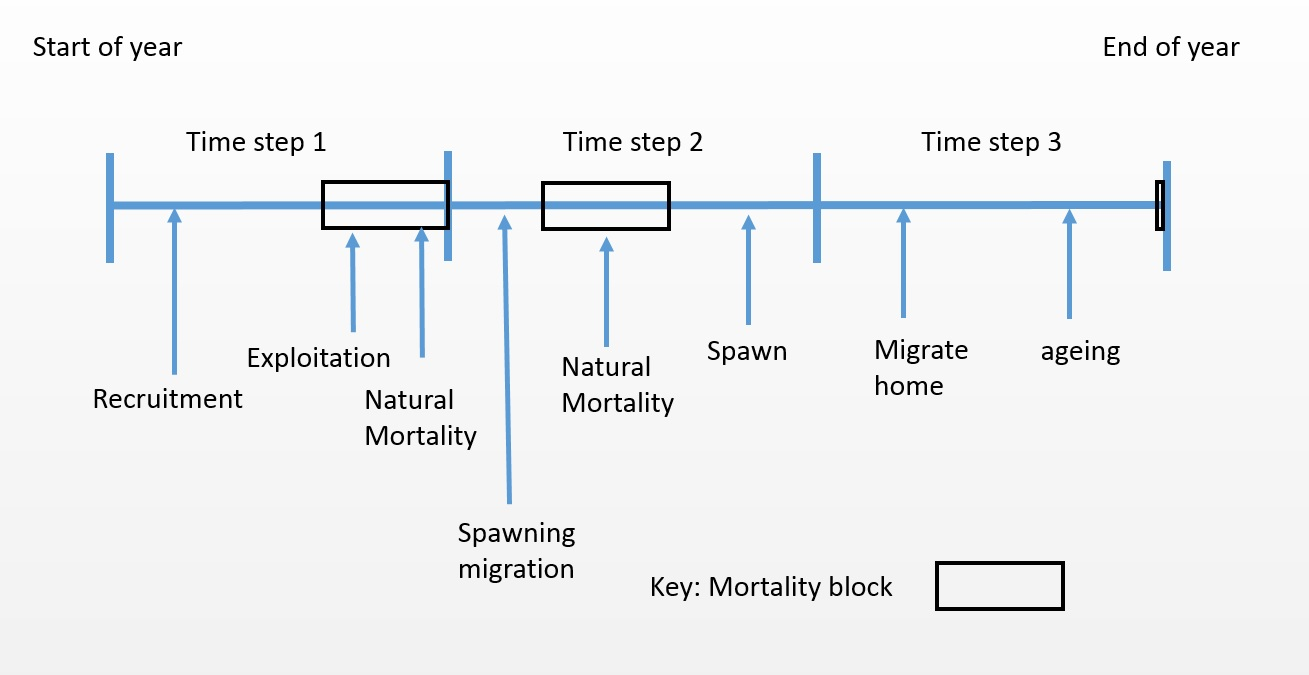
\includegraphics[scale=0.5]{Figures/annual_cycle.jpg}
	\caption{A example sequence for an annual cycle.}\label{Fig:annual2}
\end{figure}


\TODO{GO OVER M and specifying M-by-age HERE FOR ALL M-BASED PROCESSES}
\TODO{MAX U rate specification + Penalities}

\paragraph{Constant mortality rate}\label{sec:Process-MortalityConstantRate} 

To specify a constant annual mortality rate \index{Constant mortality}(e.g. $M=0.2$) for categories "male" and "female"

{\small{\begin{verbatim}
# A process with label NaturalMortality
@process NaturalMortality
type          mortality_constant_rate
categories    male female
# effectively age related mortality
relative_m_by_age One One
m             0.2 0.2
\end{verbatim}}}

The total number of individuals removed from a category

\begin{equation}
D_{j,t} = \sum_a N_{a,j,t} [1 - \exp(-S_{a,j} M_{a,j} p_t)]
\end{equation}

where $D_{j,t}$ is the total number of deaths in category $j$ in time step $t$, $N_{a,j,t}$ is the number of individuals in category $j$ of age $a$ in time step $t$, $S_{a,j}$ is the selectivity value for age $a$ in category $j$, $M_{a,j}$ is the mortality rate for category $j$ for age $a$, and $p_t$ is the proportion of the mortality rate to apply in time step $t$.

The mortality rate process requires the specification of the mortality-by-age curve which is specified using a selectivity. To apply the same mortality rate over all age classes in a category, use a selectivity defined as $S_{a,j}=1.0$ for all ages $a$ in category $j$

{\small{\begin{verbatim}
@selectivity One
type constant
c 1
\end{verbatim}}}

Age-specific mortality rates can also be applied. For example, the hypothesis that mortality is higher for younger and older individuals and lowest when individuals are at their optimal fitness could be defined by using a double exponential selectivity (see Section~\ref{sec:Selectivity})

{\small{\begin{verbatim}
@selectivity age_specific_M
type double_exponential
x0 7.06524
x1 1
x2 17
y0 0.182154
y1 1.43768
y2 1.57169
alpha 1.0

@process      NaturalMortalityByAge
type          mortality_constant_rate
categories    male female
relative_m_by_age age_specific_M age_specific_M
m             1.0 1.0
\end{verbatim}}}

\TODO{INSERT FIG OF M-by-age}

In this definition \subcommand{m} is set to 1.0 and the rate is described through the selectivity. Otherwise, $M_{age} = S_{age} * m$. This concept can be constructed similarly for other mortality methods such as \subcommand{instantaneous\_mortality}.

\paragraph{Event and biomass-event mortality}\label{sec:Process-MortalityEvent}\label{sec:Process-MortalityEventBiomass} \STATUS{Untested?}

\TODO{WHEN NOT DOING M and FISHING AT THE SAME TIME}

The event mortality\index{Event mortality} and biomass-event mortality\index{Biomass-event mortality} processes are applied in a similar manner, except that they remove a specified abundance (number of individuals) or biomass, respectively. These mortality processes can be used to define mortality events where the numbers of removals are known, e.g., fishing, rather than applying mortality as a rate.

In these cases, the abundance or biomass removed is also constrained by a maximum exploitation rate. \CNAME\ removes as many individuals or as much biomass as possible,  while not exceeding the maximum exploitation rate.

Event mortality processes require a penalty to avoid estimating parameter values that will not allow the defined number of individuals to be removed. The model penalises those parameter estimates that result in an too low a number of individuals in the defined categories (after applying selectivities) to allow for removals at the maximum exploitation rate, with a similar penalty for biomass. See Section \ref{sec:Penalty} for more information on how to specify penalties.

The event mortality applied to user-defined categories $i$, with the numbers removed at age $j$ determined by a selectivity-at-age $S_j$:

First, calculate the vulnerable abundance for each category $j$ in $1 \ldots J$ for ages $a = 1 \ldots A$ that are subject to event mortality

\begin{equation}
  V_{a,j} = S_{a,j} N_{a,j}
\end{equation}

and define the total vulnerable abundance $V_{total}$ as

\begin{equation}
  V_{total}  = \sum\limits_j {\sum\limits_a {V_{a,j}}}
\end{equation}

The exploitation rate\index{Maximum exploitation rate} to apply is

\begin{equation}
U = \begin{cases}
  C/V_{total}, & \text{if $C/V_{total} \leq U_{max}$} \\
  U_{max}, & \text{otherwise}\\
  \end{cases}
\end{equation}

The number removed $R_{a,j}$ from each age $a$ in category $j$ is,

\begin{equation}
  R_{a,j} = U V_{a,j}
\end{equation}

For example, to specify an \textbf{abundance-based} fishing mortality process with catches given for a set of specific years over categories "immature" and "mature", with selectivity "FishingSel", and assuming a maximum possible exploitation rate of 0.7, the syntax is

{\small{\begin{verbatim}
	@process     Fishing
	type          event_mortality
	categories    immature mature
	years         2000 2001 2002 2003
	U_max         0.70
	selectivities FishingSel FishingSel
	penalty       event_mortality_penalty
	\end{verbatim}}}

and specified similarly for a \textbf{biomass-based} fishing mortality process

{\small{\begin{verbatim}
		@process      Fishing
		type          mortality_event_biomass
		categories    immature mature
		years         2000 2001 2002 2003
		U_max         0.70
		selectivities FishingSel FishingSel
		penalty      event_mortality_penalty
		\end{verbatim}}}

\paragraph{Instantaneous mortality}\label{sec:Process-MortalityInstantaneous}\label{sec:Process-MortalityInstantaneousEventBiomass}\label{sec:Process-MortalityInstantaneousEvent}

The instantaneous mortality process\index{Instantaneous mortality} combines both natural mortality and fishing exploitation into a single process. This allows the simultaneous application of both natural mortality and anthropogenic mortality to occur across multiple time steps. This process accounts for half the natural mortality within a time step before calculating vulnerable biomasses for calculating exploitation rates. The remaining half of the natural mortality is taken after exploitation has been accounted for. The input for this process is catches and these can either be specified as biomasses or numbers (abundance). In fisheries models in \CNAME\ this is the most commonly used mortality process.

This process allows for multiple removal events, e.g., a fisheries model with multiple fisheries and/or fleets. A removal method can occur in one time step only, although multiple removals can be defined to cover events during the year.

The equations for instantaneous mortality are based on popes discrete catch equation, it assumes catch is known without error and \CNAME\ will try and take the exact catch in the input.

\TODO{redo equations, as notation is not consistent with that above, e.g., $S_{a,j}$}

\begin{itemize}
	\item An exploitation rate (actually a proportion) is calculated for each fishery, as the catch divided by the selected-and-retained abundance or biomass),
	$$ U_f = \frac{C_f}{\sum_a \bar{w}_a S_{f,a} n_a exp(-0.5 t M_a)}$$
	\item The mortality pressure associated with method $f$ is defined as the maximum proportion of fish taken from any element of the partition in the area affected by the method $f$
	$$ U_{f,obs} = max_a(\sum_k S_{k,a} U_k) $$
	where the maximum is over all partition elements affected by fishery $f$, and the summation is over all methods $k$ which affect the $j$th partition element in the same time step as fishery $f$.

	In most cases the mortality pressure will be equal to the exploitation rate (i.e., $U_{f,obs} = U_f$), but can be different if: (a) there is another removal method operating in the same time step as removal method $f$ and affecting some of the same partition elements, and/or (b) the selectivity $S_{f,a}$ does not have a maximum value of 1.

	There is a maximum mortality pressure limit of $U_{f,max}$ for each method of removal $f$. So, no more than proportion $U_{f,max}$ can be taken from any element of the partition affected by removal method $f$ in that time step. Clearly, $0 \leq U_{max} \leq 1$. It is an error if two removal methods, which affect the same partition elements in the same time step, do not have the same $U_{max}$.

	For each $f$, if $U_{f,obs} > U_{f,max}$, then $U_f$ is multiplied by $U_{f,max}/U_{f,obs}$ and the mortality pressures are recalculated. In this case the catch actually taken from the population in the model will differ from the specified catch, $C_f$.

	\item The partition is updated using
		$$ n'_a = n_a exp(-tM_a)\big[1 - \sum_f S_{f,a} U_f \big] $$
\end{itemize}

For example, to apply natural mortality of $0.20$ across three time steps on both male and female categories, with two methods of removals (fisheries \texttt{FishingWest} and \texttt{FishingEast}) and their respective catches (kg) known for years 1975:1977 (the catches are given in the \texttt{catches} table and information on selectivities, penalties, and maximum exploitation rates are given in the \texttt{method} table), the syntax is

\TODO{where is \texttt{time\_step\_ratio} and its usage defined?}

{\small{\begin{verbatim}
	@process instant_mort
	type mortality_instantaneous
	m 0.20
	time_step_proportions 0.42 0.25 0.33
	relative_m_by_age One
	categories male female
	biomass true
	units kgs

	table catches
	year FishingWest FishingEast
	1975	80000	111000
	1976	152000	336000
	1977	74000	1214000
	end table

	table method
	method       category  selectivity u_max   time_step  penalty
	FishingWest   stock     westFSel    0.7     step1     CatchPenalty
	FishingEast   stock     eastFSel    0.7     step1     CatchPenalty
	end_table
	\end{verbatim}}}

and for referencing catch parameters for use in projecting, time-varying, and estimating, the syntax is

{\small{\begin{verbatim}
		parameter process[mortality_instantaneous].method_"method_label"{2018}
\end{verbatim}}}

where \subcommand{"method\_label"} is the label from the \subcommand{catch} or \subcommand{method} table and continuing the example,

{\small{\begin{verbatim}
		parameter process[instant_mort].method_FishingWest{2018}
\end{verbatim}}}

To calculate weight by empirical weight-at-age matrices as described in Section~\ref{sec:AgeWeight}, the method table would include an additional column to reference weight-at-age objects:

{\small{\begin{verbatim}
		@age_weight jan_weight_at_age
		type data
		table data
		year 1 		2 		3 		4
		1980 3.4	5.6		7.23 	8.123
		end_table

		table method
		method       category  selectivity  u_max  time_step  penalty       age_weight
		FishingWest  stock     westFSel     0.7    step1      CatchPenalty  jan_weight_at_age
		FishingEast  stock     eastFSel     0.7    step1      CatchPenalty  jan_weight_at_age
		end_table
\end{verbatim}}}


\paragraph{Instantaneous mortality with retained catch and discards}\label{sec:Process-MortalityInstantaneousRetained}

The instantaneous mortality retained process\index{Instantaneous mortality retained} builds on the instantaneous mortality process (\ref{sec:Process-MortalityInstantaneous}) which has simultaneous applications of fishing and natural mortality, but with all catch-at-sea being landed, i.e., no discarding. The process \texttt{mortality\_instantaneous\_retained} allows for retained catch, discards, and also a mortality to be applied to discards, i.e., some are allowed to survive. The method for taking catch from the partition and the constraints used are the same as in \texttt{mortality\_instantaneous}.

This process was implemented to address issues with the pot fishery for blue cod which has a minimum legal size and so some catch is discarded at sea and some of these discards are expected to survive (based on some experimental work). There are length data taken at sea, so the total catch selectivity can be estimated, and length and age data taken from the landed catch (retained), so the retention selectivity can also be estimated.

In this mortality process, discard mortality is specified by defining a selectivity to represent mortality by age or length (e.g., constant or asymptotic descending logistic).  This discard selectivity is not be estimated since there is no observation class associated with it. If discard mortality is not provided, it is assumed that all discards die. Landed catch, and both the retained and total catch selectivities must be specified.

Extending the example shown in instantaneous mortality process (\ref{sec:Process-MortalityInstantaneous}) to use retained weight instead of catch, the commands are:

{\small{\begin{verbatim}
@process FishingRetainedCatch
type mortality_instantaneous_retained
# natural mortality
m 0.20
# the ratio of natural mortality in each of the three time steps
time_step_proportions 0.42 0.25 0.33
relative_m_by_age One
#for natural mortality by age
categories male female
units kgs

table catches
# two fisheries, West and East
year FishingWest FishingEast
# the catches are now landed catch
1975 80000 111000
1976 152000 336000
1977 74000 1214000
end table

table method
# all discards die
method   category selectivity retained_selectivity u_max time_step      penalty
FishingWest stock    westFSel      westRetainedSel   0.7     step1 CatchPenalty
FishingEast stock    eastFSel      eastRetainedSel   0.7     step1 CatchPenalty
end_table
\end{verbatim}}}

If discard mortality is less than 1.0, use:

{\small{\begin{verbatim}
table method
# 50% discard mortality
method   category selectivity retained_selectivity discard_mortality u_max time_step penalty
FishingWest stock  westFSel    westRetainedSel         DisMort        0.7 step1 CatchPenalty
FishingEast stock  eastFSel    eastRetainedSel         DisMort        0.7 step1 CatchPenalty
end_table

@selectivity DisMort
Type constant
# 50% mortality of discards
c 0.5
\end{verbatim}}}

See the instantaneous mortality process (\ref{sec:Process-MortalityInstantaneous}) for referencing catch parameters and calculating weight using empirical weight-at-age matrices.

The report outputs total catch, actual landed catch, and discards, without and with discard mortality:

{\small{\begin{verbatim}
@report Mortality
type process
process Instantaneous_Mortality_Retained
\end{verbatim}}}

\TODO{redo notation, as it is not consistent with that above, e.g., $S_{a,j}$ and $R_y$}

In the following, fisheries are indexed by $f$, and $a$ indexes both age and category combinations.

The total catch is found by applying a selectivity, $S_{f,a}$, in the same way as in the instantaneous mortality process. Retention, $R_{f,a}$, is defined by specifying a selectivity, which can be a function of length or age. The retained catch is the product of these two values, $R_{f,a} * S_{f,a}$. If sex is in the partition, then there are potentially two retention curves, one for each sex.

In general, there is a retention curve for each category in the partition. This property does not apply to surveys. Discard mortality is also specified as a selectivity, $D_{f,a}$. The fraction of dead fish from fishing activity is $S_{f,a} * [ R_{f,a} + (1.0 - R_{f,a}) * D_{f,a} ]$. If $D_{f,a}$ is 1.0, then all selected fish are dead, and if it is 0.0, then only the retained fish are dead.

The equations for the \texttt{mortality\_instantaneous\_retained} process:

\begin{itemize}
    \item Total catch (catch-on-board), $C_{f}$, is calculated by (retained catch) * VF / VR, where VF is vulnerable retained biomass, $j$ indexes categories and $t$ is the proportion of M in the time step, and VF is the full vulnerable biomass, $VF = \sum_{a,j} \overline{w}_{a} S_{a,j} n_{a,j} \exp(-0.5 t M_{a,j})$.

    \item An exploitation rate (actually a proportion) is calculated for each fishery, as the total catch (retained + discards) divided by the selected biomass (VF above) using selectivity $S_{f,a}$,
        $$ U_f = \frac{C_f}{\sum_a \bar{w}_a S_{f,a} n_a \exp(-0.5 t M_{a})}$$

    \item The mortality pressure associated with method $f$ is defined as the maximum proportion of fish taken from any element of the partition in the area affected by the method $f$,
        $$ U_{f,obs} = max_a (\sum_k S_{k,a} U_k) $$
    where the maximum is over all partition elements affected by fishery $f$, and the summation is over all methods $k$ which affect the $j$th partition element in the same time step as fishery $f$.

    In most cases the mortality pressure will be equal to the exploitation rate (i.e., $U_{f,obs} = U_f$), but can be different if: (a) there is another removal method operating in the same time step as removal method $f$ and affecting some of the same partition elements, and/or (b) the selectivity $S_{f,a}$ does not have a maximum value of 1.

    There is a maximum mortality pressure limit of $U_{f,max}$ for each method of removal $f$. So, no more than proportion $U_{f,max}$ can be taken from any element of the partition affected by removal method $f$ in that time step. Clearly, $0 \leq U_{max} \leq 1$. It is an error if two removal methods, which affect the same partition elements in the same time step, do not have the same $U_max$.

    For each $f$, if $U_{f,obs} > U_{f,max}$, then $U_f$ is multiplied by $U_{f,max}/U_{f,obs}$ and the mortality pressures are recalculated. In this case the catch actually taken from the population in the model will differ from the specified catch, $C_f$.

    \item Discard numbers-at-age (including their share of natural mortality) is $S_{a,j} (1 - R_{a,j}) n_{a,j} \exp(-0.5 t M_{a,j})$, and those that die at the end of the time step (updating the partition) are $D_{a,j} S_{a,j} (1 - R_{a,j}) n_{a,j} \exp(-t M_{a,j})$, where $D_{f,a}$ is the fraction that die on return to the sea.

    \item The partition is updated by removing landed catch, natural mortality, and discard mortality
        $$ n'_{a} = n_{a} \exp(-t M_a) \big[ 1 - \sum_f S_{f,a} U_f (R_{f,a} + D_{f,a} (1 - R_{f,a})) \big] $$
\end{itemize}

\paragraph{\I{Holling mortality rate}}\label{sec:Process-MortalityHollingRate} \STATUS{Untested}

The density-dependent Holling mortality process\index{Holling mortality} applies the Holling Type II or Type III functions \citep{Holling1959}, and is generalised by the Michaelis-Menten equation \citep{MentenMichaelis1913}.

This mortality process removes a number or biomass from a set of categories according to the total (selected) abundance (or biomass) and some "predator" abundance (or biomass), and is constrained by a maximum exploitation rate.

The mortality applied to user-defined categories $k$, with the numbers removed at age $l$, determined by a selectivity-at-age $S_l$ is applied as follows:

First, calculate the total predator abundance (or biomass) over all predator categories $k$ in $1 \ldots K$ and ages $l = 1 \ldots L$ that are applying the mortality

\begin{equation}
	P_{k,l} = S^{predator}_l N^{predator}_{k,l}
\end{equation}

And define the total predator abundance (or biomass) $P_{total}$ as

\begin{equation}
	P_{total}  = \sum\limits_K {\sum\limits_L {P_{k,l}}}
\end{equation}

Then calculate the total vulnerable abundance (or biomass) over all prey categories $k$ in $1 \ldots K$ and ages $l = 1 \ldots L$ that are subject to the mortality

\begin{equation}
	V_{k,l} = S^{prey}_l N^{prey}_{k,l}
\end{equation}

Then define the total vulnerable abundance (or biomass) $V_{total}$ as

\begin{equation}
	V_{total}  = \sum\limits_K {\sum\limits_L {V_{k,l}}}
\end{equation}

The number to remove is then determined by

\begin{equation}
	R_{total} = P_{total} \frac{a  V_{total}^{x-1}}{b + V_{total}^{x-1}}
\end{equation}

where $x=2$ for the Holling type II function, $x=3$ for the Holling type III function, or a different value of $x \geq 1$ for the generalised Michaelis-Menten function; $a > 0$ and $b > 0$ are the Holling function parameters.

The exploitation rate\index{Maximum exploitation rate} to apply is

\begin{equation}
	U = \begin{cases}
		R_{total}/V_{total}, & \text{if $R_{total}/V_{total} \leq U_{max}$} \\
		U_{max}, & \text{otherwise}\\
	\end{cases}
\end{equation}

And the number removed $R$ from each age $l$ in category $k$ is

\begin{equation}
	R_{k,l} = U V_{k,l}
\end{equation}

The density-dependent Holling mortality process is applied either as a function of biomass or abundance, depending on the value of the \texttt{is\_abundance} switch.

For example, a biomass Holling type II mortality process on prey \texttt{prey} by predator \texttt{predator} has the syntax

{\small{\begin{verbatim}
		@process HollingMortality
		type Holling_mortality_rate
		is_abundance F
		a 0.08
		b 10000
		x 2
		categories prey
		selectivities One
		predator_categories predator
		predator_selectivities One
		u_max 0.8
\end{verbatim}}}

\paragraph{Initialisation-event mortality}\label{sec:Process-MortalityInitialisationEvent}\label{sec:Process-MortalityInitialisationEventBiomass} \STATUS{Untested}

Initialisation event mortality\index{Initialisation event mortality} is a process that can occur only in the initialisation phase. It applies abundance or biomass mortality events specifically in initialisation phases. This option can be useful if the population is not in equilibrium before model start.

This process applies a single catch value for all iterations within the initialisation phase, and mortality will not be applied outside of the initialisation phase. This process should not be embedded in the annual cycle.

This process should be used in conjunction with the \texttt{insert\_processes} command in the \command{initialisation\_phase} block.

Example syntax where the \texttt{initialisation\_mortality\_event} has been specified in the initialisation phase \texttt{Predation\_state} but not in the annual cycle:

{\small{\begin{verbatim}
initialisation_phases Equilibrium_state Predation_state
time_steps Oct_Nov Dec_Mar

@initialisation_phase Equilibrium_state
type derived

@initialisation_phase Predation_state
type iterative
insert_processes Oct_Nov()=predation_Initialisation

@process predation_Initialisation
type initialisation_mortality_event
categories male.HOKI female.HOKI
catch 90000
selectivities Hakesl Hakesl

time_step Oct_Nov
processes Mg1 Instantaneous_Mortality

@time_step Dec_Mar
processes Recruitment Instantaneous_Mortality
\end{verbatim}}}

\paragraph{Prey-suitability mortality}\label{sec:Process-MortalityPreySuitability} \STATUS{Untested}

The density-dependent prey-suitability mortality process\index{Density-dependent prey-suitability} applies predation mortality from a predator group to its prey groups simultaneously. It removes an abundance (or biomass) from each prey group according to the total (selected) abundance (or biomass) of each prey group, the total (selected) abundance (or biomass) of the other prey groups, some "predator" abundance (or biomass), and the preference (electivity) of the predator for each prey group, constrained by a maximum exploitation rate. The predator-prey suitability functions were based on the multispecies Virtual Population Analysis (MSVPA) functions \citep{JuradoMolina2005}.

The mortality applied to the user-defined prey group $g$ of category $k$, with the numbers removed at age $l$ determined by a selectivity-at-age $S_l$ is applied as follows:

First, calculate the total predator abundance (or biomass) over all predator categories $k$ in $1 \ldots K$ and ages $l = 1 \ldots L$ that are applying the mortality

\begin{equation}
P_{k,l} = S^{predator}_l N^{predator}_{k,l}
\end{equation}

And define the total predator abundance (or biomass) $P_{total}$ as

\begin{equation}
P_{total}  = \sum\limits_K {\sum\limits_L {P_{k,l}}}
\end{equation}

Then, given the total vulnerable abundance (or biomass) of prey group $g$ over all categories $k$ in $1 \ldots K$ and ages $l = 1 \ldots L$ that are subject to the mortality

\begin{equation}
V_{g,k,l} = S^{prey}_l N^{prey}_{k,l}
\end{equation}

And define the total vulnerable abundance (or biomass) of each prey group $V^g_{total}$ as

\begin{equation}
V^g_{total}  = \sum\limits_K {\sum\limits_L {V_{g,k,l}}}
\end{equation}

And the total availability $A^g_{total}$ for each prey group as

\begin{equation}
A^g_{total} = \frac{V^g_{total}}{\sum\limits_G {V^g_{total}}}
\end{equation}

The vulnerable abundance (or biomass) and availability every prey group $g$ in $1 \ldots G$ is calculated simultaneously. Then the abundance (or biomass) to remove from each prey group $g$ is a function of its electivity $E_g$, the availability of all other prey groups $i$ in $1 \ldots G$, the electivity of the predator for each prey group $E_i$, and the total consumption rate of the predator $CR$ and its abundance (or biomass) $P_{total}$

\begin{equation}
R^g_{total}=P_{total} CR \frac{A^g_{total} E_g}{\sum\limits_G {A^i_{total} E_i}}
\end{equation}

The exploitation rate\index{Maximum exploitation rate} to apply to each prey group $g$ is then

\begin{equation}
U_g = \begin{cases}
R^g_{total}/V^g_{total}, & \text{if $R^g_{total}/V^g_{total} \leq U_{max}$} \\
U_{max}, & \text{otherwise}\\
\end{cases}
\end{equation}

And the number removed $R^g$ in each prey group $g$ from each age $l$ in category $k$ is

\begin{equation}
R_{g,k,l} = U_g V_{g,k,l}
\end{equation}

Prey suitability choice occurs only between the prey groups specified by the process. The total predator consumption rate represents the consumption of the predator on those prey groups alone. The electivities must sum to 1. Further, the consumption rate can be modified by a layer to be cell specific.

The density-dependent prey-suitability process is applied as either a biomass or an abundance depending on the value of the \subcommand{is\_abundance} switch.

Individual categories can be aggregated into prey groups using the "+" symbol. To indicate that two (or more) categories are to be aggregated, separate them with a "+" symbol.

For example, to specify two prey groups of two species made up of the males and females in each prey group

{\small{\begin{verbatim}
		prey_categories maleSpeciesA + femaleSpeciesA maleSpeciesB + femaleSpeciesB
\end{verbatim}}}

This syntax indicates that there are two prey groups, \texttt{maleSpeciesA + femaleSpeciesA} and \texttt{maleSpeciesB + femaleSpeciesB}, with each group having its own electivity.

For example, a biomass prey-suitability mortality process with an overall consumption rate of $0.8$ of prey \texttt{species A} and \texttt{species B} (modelled as males and females) by the predator \texttt{predatorSpecies} with electivities between \texttt{species A} and \texttt{species B} of $0.18$ and $0.82$ has syntax

{\small{\begin{verbatim}
		@process PreySuitabilityMortality
		type prey-suitability_predation
		is_abundance F
		consumption_rate 0.8
		categories maleSpeciesA + femaleSpeciesA maleSpeciesB + femaleSpeciesB
		electivities 0.18 0.82
		selectivities One One One One
		predator_categories predatorSpecies
		predator_selectivities One
		u_max 0.8
\end{verbatim}}}

\subsubsection{\I{Transition By Category}}\label{sec:Process-TransitionCategory}

The transition by category process moves individuals between categories. This process is used to specify transitions such as maturation (individuals move from an immature to mature state) and migration (individuals move from one area to another).

There is a one-to-one relationship between the "from" category and the "to" category, i.e., for every source category there is one target category only

\begin{equation}
	N_{a,j} = N_{a,i} \times P_i \times S_{a,i}
\end{equation}

where $N_{a,j}$ is the number of individuals that have moved to category $j$ from category $i$ in age $a$, $N_{a,i}$ is the number of individuals in category $i$, $P_i$ is the proportion parameter for category $i$, and $S_{a,i}$ is the selectivity at age $a$ for category $i$.

To merge categories repeat the "to" category multiple times.

For example, to specify a simple spawning migration of mature males from a western area to an eastern (spawning) area, the syntax is

{\small{\begin{verbatim}
		@process Spawning_migration
		type transition_category
		from West.males
		to East.males
		selectivities MatureSel
		proportions 1
		\end{verbatim}}}

where \texttt{MatureSel} is a selectivity that describes the proportion of age or length classes that are mature and thus move to the eastern area.

\paragraph{Transition by category by age}\label{sec:Process-TransitionCategoryByAge}

A special process type is the transition by category by age process, which allows a transition to occur for a specific subset of ages in specific years only, where each year can have a different number that are moved between categories.

\subsubsection{\I{Tag Release events}}\label{sec:Process-TagByAge}\label{sec:Process-TagByLength} 

Tagging processes can be age- or length-based processes, whereby numbers of individuals are moved from an untagged category to a tagged category defined in the \command{categories} block. Tag release processes can also account for initial tag-induced mortality on individuals.

Age-based tag release events move a known number of individuals tagged for each age to a tagged category, along with applying additional mortality. Individuals are removed from the non-tagged categories and added to tagged categories. Often the ages of tagged individuals are not known, so length-based tag release events are more commonly used.

Length-based tag release processes are more complicated, as the age-length matrix is calculated and the exploitation for each length bin to then move the correct numbers-at-age based on the known lengths of release. \CNAME\ also allows for initial tag loss.


\paragraph*{{Tag Release By Length}}
\subcommand{compatability\_switch casal2}\\

For each length bin $l$ of the input vector of proportions-at-length ${p}_l$ and total tag releases denoted by \(M\). The vulnerable numbers for age \(a\), length \(l\), and category \(j\) are calculated as
$$V_{a,l,j} = N_{a,j} \phi_{a,l,j} S_{a,j}$$
where, \(\phi_{a,l,j}\) is the age-length matrix (Section~\ref{sec:AgeLength-length_at_age}), and \(S_{a,j}\) is the selectivity. The transition matrix is calculated as,
$$ T_{a,l,j}= \frac{V_{a,l,j}}{\sum_a\sum_j V_{a,l,j}} {p}_l$$
and final tag-release by age and category are
$$ M_{a,j} = \sum_l T_{a,l,j}M  $$
An age based maximum transition rate is calculated to stop tagging more fish than are available in the population, in this case the penalty is flagged, see below
$$ u_{a,j} = \frac{ M_{a,j} }{N_{a,j} }  $$

$$
u_{a,j} =
\begin{cases}
u_{max},& \text{if } u_{a,j} > u_{max} \text{ \textbf{flag a penalty}}\\
u_{a},  & \text{otherwise}
\end{cases}
$$

The resulting tag-releases for each age and category denoted by \(\widetilde{N}_{a,j}\) are thus,
$$
\widetilde{N}_{a,j} = N_{a,j} u_{a,j}
$$

Release mortality denoted by \(h_a\) can also be applied as,

$$\widetilde{N}_{a,j} = \widetilde{N}_{a,j}\left(1.0 - h_a\right)$$


The syntax for an example of tag release by length process
{\small{\begin{verbatim}
@process 2005Tags_shelf
type tag_by_length
years 2005
from male.untagged+female.untagged
to male.2005  female.2005
selectivities ShelfselMale ShelfselFemale
penalty tagging_penalty
initial_mortality 0.1
table proportions
year 30 40 50 60 70 80 90 100 110 120 130 140 150 160 170 180 190 200 210 220
2005  0 0 0.0580 0.1546 0.3380 0.1981 0.1643 0.0531 0.0242 0.0097 0 0 0 0 0 0 0 0 0 0
end_table
n 207
U_max 0.999
\end{verbatim}}}

This process moves 207 individuals from a combination of male.untagged and female.untagged categories, based on the combination of growth rates and selectivity, into tagged male and tagged female categories.


For \subcommand{compatability\_switch casal}
This describes the algorithm applied in CASAL, it should yield identical results when a single untagged category and tagged category are supplied. There is a small difference when input numbers at length are defined for a combination of categories (unsexed) and we allocated into each corresponding category (male and female). This is supplied for backwards compatibility with CASAL, we recommend using \subcommand{compatability\_switch casal2}, for when ${p}_l$ is unsexed but sex is in the partition.


For each length bin $l$ of the input vector of proportions-at-length ${p}_l$ and total tag releases denoted by \(M\). The vulnerable numbers for age \(a\), length \(l\), and category \(j\) are calculated as

$$V_{a,l} = N_{a,j} \phi_{a,l,j} S_{a,j}$$
Note this is where the \subcommand{compatability\_switch} differ, the \subcommand{casal2} option preserves the category difference, where as \subcommand{casal} amalgamates them. \(\phi_{a,l,j}\) is the age-length matrix (Section~\ref{sec:AgeLength-length_at_age}), and \(S_{a,j}\) is the selectivity. The transition matrix is calculated as,
$$ T_{a,l}= \frac{V_{a,l}}{\sum_a V_{a,l}} {p}_l$$
and final tag-release by age are
$$ M_{a} = \sum_l T_{a,l}M  $$
An age based maximum transition rate is calculated to stop tagging more fish than are available in the population, in this case the penalty is flagged, see below
$$ u_{a} = \frac{ M_{a} }{ N_{a}}  $$

$$
u_{a} =
\begin{cases}
u_{max},& \text{if } u_{a} > u_{max} \text{ \textbf{flag a penalty}}\\
u_{a},  & \text{otherwise}
\end{cases}
$$

The resulting tag-releases for each age and category denoted by \(\widetilde{N}_{a,j}\) are thus,
$$
\widetilde{N}_{a,j} = N_{a,j} u_{a}
$$
Release mortality denoted by \(h_a\) can also be applied as,

$$\widetilde{N}_{a,j} = \widetilde{N}_{a,j}\left(1.0 - h_a\right)$$


\subsubsection{\I{Tag loss}}\label{sec:Process-TagLoss} 
Tag Loss is the process which accounts for tagged fish being removed from the partition. For example tag related mortality or tag failure. This process is applied as an instantaneous mortality rate that can happen over multiple time steps in the annual cycle. This method assumes that when tags are lost the individuals are deleted from the model.


Two options are available depending on whether the tag release event were tagged with a single tag (\subcommand{tag\_type single}) and double tag (\subcommand{tag\_type double}).

For elements in the partition indexed by age \(a\) and category \(c\) , the number of tag lost (\(N^*_{c,a}\)) at time step \(t\) with loss rate \(r\) and proportion denoted by \(p^t\) for type \subcommand{single} is
\begin{equation}
	N^*_{c,a} = N_{c,a} exp\left( - r_a p^t\right)
\end{equation}
%
where \(N_{c,a}\) is the number of tagged fish before the process is applied.

For tag type \subcommand{double}
\begin{equation}
N^*_{c,a} = 1 - \left(1 - N_{c,a} exp\left( - r_a p^t\right)\right)\left(1 - N_{c,a} exp\left( - r_a p^t\right)\right)
\end{equation}
%


The syntax for the tag loss process follows
{\small{\begin{verbatim}
@process Tag_loss
type tag_loss
categories single_tagged_fish
tag_loss_rate 0.02
time_step_proportions 0.25 0.75
selectivities One
tag_loss_type single
year 1985
\end{verbatim}}}
and double tagged

{\small{\begin{verbatim}
	@process Tag_loss
	type tag_loss
	categories double_tagged_fish
	tag_loss_rate 0.02
	time_step_proportions 0.25 0.75
	selectivities One
	tag_loss_type double
	year 1985
\end{verbatim}}}